\documentclass{ximera}

\title{Examples}

\newcommand{\defnword}[1]{\textbf{#1}}
\newcommand{\ds}{\displaystyle}
\newcommand{\Z}{\mathbb{Z}}
\newcommand{\N}{\mathbb{N}}
\newcommand{\nth}{\mbox{\scriptsize th}}
\renewcommand{\index}[1]{}

\begin{document}

\begin{abstract}
  Important examples of sequences include arithmetic and geometric progressions.
\end{abstract}

\maketitle

%\marginnote{Tons of entertaining sequences are listed in the \href{http://oeis.org/}{The On-Line Encyclopedia of Integer Sequences}.}

Mathematics proceeds, in part, by finding precise statements for
everyday concepts.  We have already done this for sequences when we
found a precise definition (``function from $\N$ to $\R$'') for the
everyday concept of ``a list of real numbers.''  But all the
formalisms in the world aren't worth the paper they are printed on if
there aren't some interesting \textit{examples} of those precise
concepts.  Indeed, mathematics proceeds not only by generalizing and
formalizing, but also by focusing on specific, concrete instances.
So let me share some specific examples of sequences.

But before I can share these examples, let me address a question: how
can I hand you an example of a sequence? It is not enough just to list
off the first few terms.  Let's see why.

\begin{question}
  Consider the sequence $(a_n)$
  $$
  a_1 = 41, \quad a_2 = 43, \quad a_3 = 47, \quad a_4 = 53, \quad\ldots
  $$
  What is the next term $a_5$?  Can you identify the sequence?

  \begin{solution}
    \begin{multiple-choice}
      \choice[correct]{No}
      \choice{Yes}
    \end{multiple-choice}  
  \end{solution}
  
  In spite of many so-called ``intelligence tests'' that ask questions
  just like this, this question simply doesn't have an answer.  Or
  worse, it has too many answers!
   
  This sequence might be ``the prime numbers in order, starting at
  41.''  If that's the case, then the next term is $a_5 =59$.  But
  maybe this sequence is the sequence given by the polynomial $a_n =
  n^2 - n + 41$.  If that's the case, then the next term is $a_5 =
  61$.  Who is to say which is the ``better'' answer?
\end{question}

Now let's consider two popular ``families'' of sequences and some popular examples.


\subsection{Triangular numbers}

The sequence of \defnword{triangular numbers} $(T_n)$ is a sequence of
integers counting the number of dots in increasingly large
``equilateral triangles'' built from dots.  The term $T_n$ is the
number of dots in a triangle with $n$ dots to a side.

\begin{fullwidth}
\begin{figure*}[!h]
\begin{minipage}{0.6in}
\begin{center}

\begin{tikzpicture}[y=0.5cm,x=0.3415cm]
\fill (0,0) circle (3pt);
\end{tikzpicture} \\
$T_1 = 1$
\end{center}
\end{minipage}
\begin{minipage}{1.1in}
\begin{center}
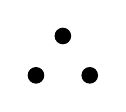
\begin{tikzpicture}[y=0.5cm,x=0.3415cm]
\fill (0,0) circle (3pt);
\fill (1,-1) circle (3pt);
\fill (-1,-1) circle (3pt);
\end{tikzpicture} \\
$T_2 = 3$
\end{center}
\end{minipage}
\begin{minipage}{1.2in}
\begin{center}
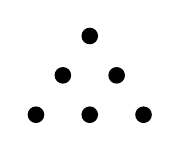
\begin{tikzpicture}[y=0.5cm,x=0.3415cm]
\fill (0,0) circle (3pt);
\fill (1,-1) circle (3pt);
\fill (-1,-1) circle (3pt);
\fill (-2,-2) circle (3pt);
\fill (0,-2) circle (3pt);
\fill (2,-2) circle (3pt);
\end{tikzpicture} \\
$T_3 = 6$
\end{center}
\end{minipage}
\begin{minipage}{1.3in}
\begin{center}
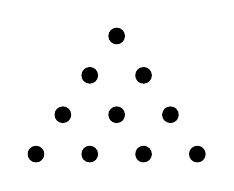
\begin{tikzpicture}[y=0.5cm,x=0.3415cm]
\fill (0,0) circle (3pt);
\fill (1,-1) circle (3pt);
\fill (-1,-1) circle (3pt);
\fill (-2,-2) circle (3pt);
\fill (0,-2) circle (3pt);
\fill (2,-2) circle (3pt);
\fill (-3,-3) circle (3pt);
\fill (-1,-3) circle (3pt);
\fill (1,-3) circle (3pt);
\fill (3,-3) circle (3pt);
\end{tikzpicture} \\
$T_4 = 10$
\end{center}
\end{minipage}
\begin{minipage}{1.5in}
\begin{center}
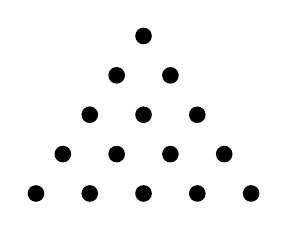
\begin{tikzpicture}[y=0.5cm,x=0.3415cm]
\fill (0,0) circle (3pt);
\fill (1,-1) circle (3pt);
\fill (-1,-1) circle (3pt);
\fill (-2,-2) circle (3pt);
\fill (0,-2) circle (3pt);
\fill (2,-2) circle (3pt);
\fill (-3,-3) circle (3pt);
\fill (-1,-3) circle (3pt);
\fill (1,-3) circle (3pt);
\fill (3,-3) circle (3pt);
\fill (-4,-4) circle (3pt);
\fill (-2,-4) circle (3pt);
\fill (0,-4) circle (3pt);
\fill (2,-4) circle (3pt);
\fill (4,-4) circle (3pt);
\end{tikzpicture} \\
$T_5 = 15$ \\
\end{center}
\end{minipage}
\begin{minipage}{1.7in}
\begin{center}
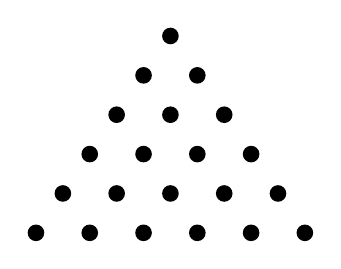
\begin{tikzpicture}[y=0.5cm,x=0.3415cm]
\fill (0,0) circle (3pt);
\fill (1,-1) circle (3pt);
\fill (-1,-1) circle (3pt);
\fill (-2,-2) circle (3pt);
\fill (0,-2) circle (3pt);
\fill (2,-2) circle (3pt);
\fill (-3,-3) circle (3pt);
\fill (-1,-3) circle (3pt);
\fill (1,-3) circle (3pt);
\fill (3,-3) circle (3pt);
\fill (-4,-4) circle (3pt);
\fill (-2,-4) circle (3pt);
\fill (0,-4) circle (3pt);
\fill (2,-4) circle (3pt);
\fill (4,-4) circle (3pt);
\fill (-5,-5) circle (3pt);
\fill (-3,-5) circle (3pt);
\fill (-1,-5) circle (3pt);
\fill (1,-5) circle (3pt);
\fill (3,-5) circle (3pt);
\fill (5,-5) circle (3pt);
\end{tikzpicture} \\
$T_6 = 21$ \\
\end{center}
\end{minipage}
\vspace{12pt}

\caption{The first six triangular numbers}
\end{figure*}
\end{fullwidth}

There are a couple of ways of making this discussion more precise.
Given an equilateral triangle with $n$ dots to a side, how many more
dots do you need to build the equilateral triangle with $n+1$ dots to
a side?  All you need to do to transform the smaller triangle to the
larger triangle is an additional row of $n+1$ dots placed along any
side.  Therefore,
\[
T_{n+1} = T_n + (n+1).
\]
Since $T_1 = 1$, this recursive definition suffices to determine the
whole sequence.

But there are other ways of computing $T_n$.  Indeed, you may recall
the explicit formula
$$
T_n = \frac{n \cdot (n+1)}{2}
$$
from Calculus One.

\subsection{Fibonacci numbers}

%\marginnote{The Fibonacci numbers are interesting enough that a
%  journal, \href{http://www.fq.math.ca/}{The Fibonacci Quarterly} is
%  published four times yearly entirely on topics related to the
%  Fibonacci numbers.}

The \defnword{Fibonacci numbers} are defined recursively, starting with
$$
F_0 = 0 \mbox{ and } F_1 = 1
$$
and the rule that $F_{n} = F_{n-1} + F_{n-2}$.  We can restate this
formula in words, instead of symbols; stated in words, each term is
the sum of the previous two terms.  So the sequence of Fibonacci
numbers begins 
$$
0, \quad 1, \quad 1, \quad 2, \quad 3, \quad 5, \quad 8, \quad 13, \quad 21, \quad 34, \quad\ldots
$$
and continues.

This is certainly not the last time we will see the Fibonacci numbers.

\subsection{Collatz sequence}

Here is a fun sequence with which to amuse your friends---or distract
your enemies.  Let's start our sequence with $a_1 = 6$.  Subsequent
terms are defined using the rule
$$
a_n = \begin{cases} a_{n-1} / 2 & \mbox{ if $a_{n-1}$ is even, and } \\
3 \, a_{n-1} + 1 & \mbox{ if $a_{n-1}$ is odd.}
\end{cases}
$$
Let's compute $a_2$.  Since $a_1$ is even, we follow the instructions
in the first line, to find that $a_2 = a_1/2 = 3$. To compute $a_3$,
note that $a_2$ is odd so we follow the instruction in the second
line, and $a_3 = 3 \, a_2 + 1 = 3 \cdot 3 + 1 = 10$.  Since $a_3$ is
even, the first line applies, and $a_4 = a_3 / 2 = 10 / 2 = 5$.  But
$a_4$ is odd, so the second line applies, and we find $a_5 = 3 \cdot 5
+ 1 = 16$.  And $a_5$ is even, so $a_6 = 16 / 2 = 8$.  And $a_6$ is
even, so $a_7 = 8/4 = 4$.  And $a_7$ is even, so $a_8 = 4 / 2 = 2$,
and then $a_9 = 2/2 = 1$.  Oh, but $a_9$ is odd, so $a_{10} = 3 \cdot
1 + 1 = 4$.  And it repeats.  Let's write down the start of this sequence:
$$
6,\quad %1 
3,\quad %2
10,\quad  %3
5,\quad  %4
16,\quad  %5
8,\quad  %6
4,\quad  %7
2,\quad  %8
1,\quad  %9
4,\quad %10
2,\quad %11
1,\quad %12
\overbrace{4,\quad %10
2,\quad %11
1,}^{\mbox{repeats}}\quad %12
4,\quad %10
\ldots
$$
What if we had started with a number other than six?  What if we set
$a_1 = 25$ but then we used the same rule?  In that case, since $a_1$
is odd, we compute $a_2$ by finding $3 \, a_1 + 1 = 3 \cdot 25 + 1 =
76$.  Since $76$ is even, the next term is half that, meaning $a_3 =
38$.  If we keep this up, we find that our sequence begins
\begin{align*}
&25,\quad 76,\quad 38,\quad 19,\quad 58,\quad 29,\quad 88,\quad 44,\quad 22,\quad 11,\quad 34,\quad 17,\quad 52,\quad 26, \\
&13,\quad 40,\quad 20,\quad 10,\quad 5,\quad 16,\quad 8,\quad 4,\quad 2, \quad 1, \quad \ldots
\end{align*}
and then it repeats ``4, 2, 1, 4, 2, 1, \ldots'' just like before.

\marginnote{If you think you have an argument that answers the Collatz conjecture, I challenge you to try your hand at the $5x+1$ conjecture, that is, use the rule
$
a_n = \displaystyle\begin{cases} a_{n-1} / 2 & \mbox{ if $a_{n-1}$ is even, and } \\
5 \, a_{n-1} + 1 & \mbox{ if $a_{n-1}$ is odd.}
\end{cases}
$}

Does this always happen?  Is it true that no matter which positive
integer you start with, if you apply the half-if-even, $3x+1$-if-odd
rule, you end up getting stuck in the ``4, 2, 1, \ldots'' loop?  That
this is true is the \defnword{Collatz conjecture}; it has been
verified for all starting values below $5 \times 2^{60}$.  Nobody has
found a value which doesn't return to one, but for all anybody knows
there \textit{might} well be a very large initial value which doesn't
return to one; nobody knows either way.  It is an unsolved
problem\sidenote{This is not the last unsolved problem we will
  encounter in this course.  There are many things which humans do not
  understand.} in mathematics.

\end{document}
